% The model under study: a linear encoder 4 -> 2 followed by a stack of bilinear MLPs.
% Compile from figures/ (the fonts resolve relative to the cwd): lualatex setup_diagram.tex,
% then pdftoppm -png -r 200 and autocrop to setup_diagram.png (see ../reproduce.sh).
\documentclass{article}
\usepackage[a4paper, margin=1cm]{geometry}
\pagestyle{empty}
\usepackage{fontspec}
\usepackage{xcolor}
\usepackage{amsmath}
\usepackage{tikz}
\setmainfont{Poppins}[
  Path = fonts/Poppins/,
  Extension = .ttf,
  UprightFont = *-Regular,
  BoldFont = *-Bold,
  ItalicFont = *-Italic,
  BoldItalicFont = *-BoldItalic
]
\definecolor{pivotalOrange}{HTML}{F15F22}
\definecolor{pivotalBlue}{HTML}{3A82B5}
\definecolor{pivotalTaupe}{HTML}{818089}
\tikzset{
  lbl/.style={font=\fontsize{17}{20}\selectfont},
  sm/.style={font=\fontsize{14}{17}\selectfont},
}
\begin{document}
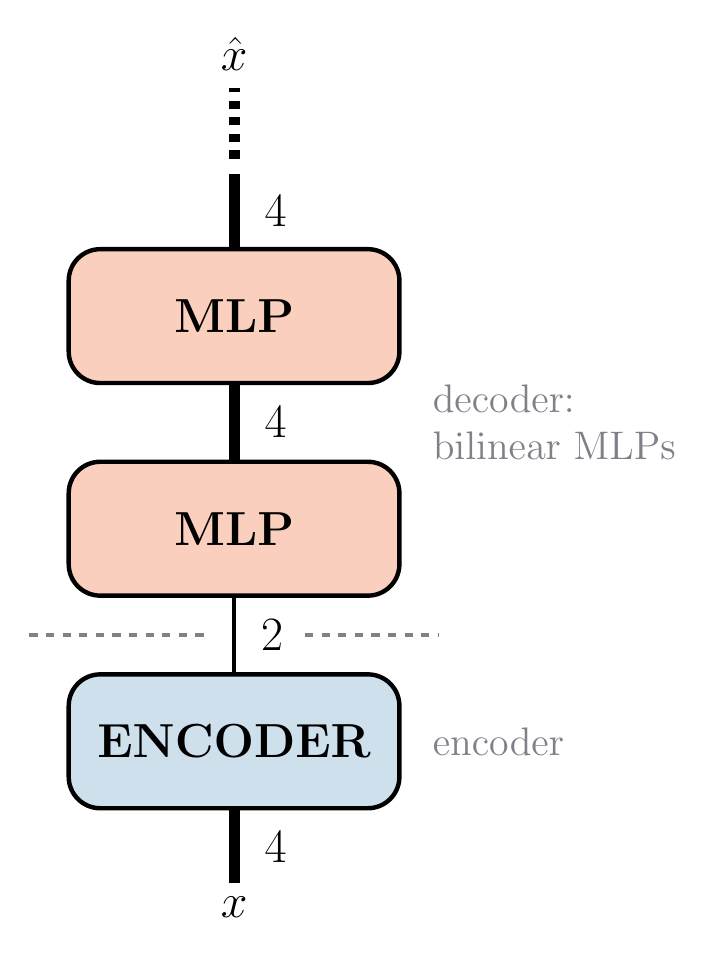
\begin{tikzpicture}[
  block/.style={draw, line width=1.6pt, rounded corners=4mm, minimum width=4.2cm,
                minimum height=1.7cm, font=\bfseries\fontsize{18}{22}\selectfont},
  wide/.style={line width=4pt}, narrow/.style={line width=1.6pt}, lbl]
  \node[block, fill=pivotalBlue!25]   (enc)  at (0,0)   {ENCODER};
  \node[block, fill=pivotalOrange!30] (mlpa) at (0,2.7) {MLP};
  \node[block, fill=pivotalOrange!30] (mlpb) at (0,5.4) {MLP};
  \draw[wide]   (0,-1.8) -- (enc.south)     node[midway, right=2mm] {4};
  \draw[narrow] (enc.north) -- (mlpa.south)  node[midway, right=2mm] {2};
  \draw[wide]   (mlpa.north) -- (mlpb.south) node[midway, right=2mm] {4};
  \draw[wide]   (mlpb.north) -- (0,7.2)      node[midway, right=2mm] {4};
  \draw[wide, dashed] (0,7.4) -- (0,8.3);
  \node[below] at (0,-1.85) {$x$};
  \node[above] at (0,8.4)   {$\hat{x}$};
  \draw[dashed, pivotalTaupe, line width=1.2pt] (-2.6,1.35) -- (-0.3,1.35);
  \draw[dashed, pivotalTaupe, line width=1.2pt] (0.9,1.35) -- (2.6,1.35);
  \node[right, pivotalTaupe, sm] at (2.4,0) {encoder};
  \node[right, pivotalTaupe, sm, align=left] at (2.4,4.05) {decoder:\\ bilinear MLPs};
\end{tikzpicture}
\end{document}
